\documentclass{ltjsbook}
\usepackage{docmute} 
\usepackage{../../myStyle} 

\begin{document}
\setcounter{chapter}{3}
\chapter{社会心理学の歴史3;社会心理学の萌芽}
\label{sp04_history1}
\section{前回の振り返り；人文知と客観性}
それでは時間になりましたのでお話を始めたいと思います。前回のコメントの振り返りからいきたいのですが，その思想の歴史について，自学では厳しいと思っていたのでまとめがあってよかったというご意見もいただきましたし，分からないというご意見もいただきました。申し訳ありません，たぶん私の説明が不十分，あるいは本質を理解しきれていないのか，伝えきれていないのかと思います。私の話は皆さんが考えるものの入り口になってくれればと思いますので，私の話で何か引っかかりがあったら，ご自身で深めていっていただければと思います。

例によって講義録をとり，なるべく早くアップロードするつもりでいます。今日の授業のレジュメといいますか，こういうことを話しますというようなところは一応書いてあるものを全部LMSの方に上げていますので，確認していただければと思います。この講義録を作るときに，人名が出たときはWikipediaなどで調べて大体の概略を書くようにしています。また授業中に触れた本については引用文献をしっかりリスト化してあげるようにしています。前回のカントのお話のところについては，講義録の中ではちゃんと引用してあるのですが，一応説明しておきますと，黒崎正夫先生の『カント純粋理性批判入門』\parencite{Kurosaki2000}，これが一番分かりやすかったです。私は一番分かりやすかったので，なるほど，分からないと思われた方はこれを読んでいただくと，丁寧に説明してありますので，カントのところは理解しやすいかと思います。もちろん岩波文庫で『純粋理性批判』上・中・下巻が出ているのですが\parencite{Kant1961}，それを読んでいただいてもいいのですが，理性だけでなく悟性という単語が当然のように使われていたりして，語の定義が明確でないまま進むところもあったりします。当時のカントの時代では，そういうのがしっかり区別されて使われていたのでしょうが，説明が不足しているところもあるかと思うので，この手の入門書も悪くないというご案内です。

さて，コメントにいただいたのですが，いくつか質問があります，というのをいただきました。
まず，構成概念とモデルとの関係は何ですかというようなご質問。構成概念というのは，構成概念もモデル，理想型の一種ではあるのですが，構成概念と言われると，一般的には，一要素として全体性を持った概念のカテゴリーの枠組み，この範囲のことを概念としてまとめますよというようなところが重視されているかと思います。心理学者はそういった概念を複数使って，この概念が原因となって，この概念に影響を及ぼすだろうといったような概念の関係まで記述して議論することがあるのですが，そういったもの全体のことをモデルと言うかと思います。一応はそういう分け方で考えたらいいかと思うのですが，モデルというのも抽象化された，理想化されたものというような意味があるので，概念もモデルだし，概念間の関係も含めて記述したものもモデルです。何なら，科学というものが持っている考え方ですね。例えば，ニュートン\index[nameidx]{にゅーとん@ニュートン}が持っていた絶対空間，絶対時間というのもモデルだし，アインシュタイン\index[nameidx]{あいんしゅたいん@アインシュタイン}が考えた相対的な時空間というのもモデルです。現象学が言っているような，とりあえず究極の客観性といいますか，神の目線みたいなのをエポケー\index[termidx]{えぽけー@エポケー}しちゃって\footnote{現象学においては，エポケー\index[termidx]{えぽけー@エポケー}は世界の自然命題を「カッコに入れる」，「一旦判断を止める」ことを意味します。すなわち世界の外的現実についての信念を横に置いて，生の感覚，うけとめたその様相そのものに目を向けよ，という意味です。}，自分の目線から考えるところだけ考えましょうというふうなのも，自分というフィルターがあるよねって考えて世界を記述するモデルという言い方もできるかと思いますので，モデルの方がやや包括的な要素ではないかというふうに回答しておきたいと思います。

この方の2つ目の問いなのですが，構成概念の現象や現実へのフィックス(固定)の強さ。前回そういうふうな図を書きましたね。資料の方にちまちまとパワーポイントで絵を描いて，それを入れてありますので，見ていただきたいのですが($\to$図\ref{construct_concepts},Pp.\pageref{construct_concepts})，そのフィックスの固定の強さはどうやって評価されるのでしょうかという問いです。この方は，カッコして妥当性とか現実とモデルとの対応の解釈というふうに書いておられますね。これは難しいというか，定量化できるものではない，と言えると思います。例えば構成概念でいうところの構成概念妥当性というような言い方がありますね。そういった概念がどれぐらい妥当であるかというような言葉なのですけれども，結局のところこの妥当性というのは数値的に評価できるものではありません。

心理尺度の信頼性ということであれば，定量化できるんです。例えば再検査信頼性であれば，複数回テストした時のpre(プレ)とpost(ポスト)の相関係数の強さのとして表現できますし，内的整合性信頼性というのは項目間の全体の分散の中で，各項目同士が平均してどれぐらい分散を共有し合っているかという程度を数値化した，アルファ係数で評価ができるわけですね。アルファ係数が0.8ぐらいあればよいだろうというふうに一般的に言われたりもしますけれども，妥当性に関してはそういった数値的な判断の仕方がありません。その概念が提供された時に，「なるほど，うまいこと言っていますね」，「なるほど，それは思い当たる節がありますね」という納得の程度，話を聞かされた人の納得の程度でしかない。あるいはその概念を使ってコミュニケートするグループの，そのグループといいますか，そのコミュニティの納得の程度というところなのではないかと思います。

ずいぶん曖昧なというか，中途半端なものの言い方をするなと思われるかもしれませんけれども，前回も言いましたように，科学というのも実は，科学的な考え方，科学的な作法というのを共有し合っている人類のコミュニティに過ぎないのです。そのコミュニティの中でどれくらい普遍性あるいは妥当性といいますか，納得感があるか。「私はこういう前提で考えたらこうも言えると思うのですが，どうでしょうか」というのに，どれくらい同意できるかというところの程度として評価するしかないと思います。この辺が非科学的であるというか，客観的でないと言われたらそうなのですけれども，サイエンスあるいは科学コミュニティのパラダイムみたいなのをどう定義するかというところとも関わってきますので，それでよいのかどうかということは皆さんも考えてみてください。

特に妥当性の概念については，最近ちょっと議論が盛り上がってきています。\textcite{Kathleen2017}の訳書で，「心理学における構成概念を見つめ直す」というのが出たのですが，そこに構成概念妥当性というのが考えられてきた経緯，歴史的なバックボーンを含めての話がちゃんと載ってます。実は今まで言っていた構成概念妥当性というのは，構成概念妥当性，表面的妥当性，内容的妥当性などなど含めて，多くの妥当性のひとつだったんです。だけど，21世紀の初頭に，それ全部一緒じゃないか？ひとつの妥当性でいいんじゃないか？という意見が出てますね。いずれにせよ，きっちりした定義というのは難しい，できていないというのが現状だと思います。

それに続いての質問やコメントがあったのですが，フィックスの程度を検証するような，理論的な関係をメインに研究しているのは心理学にはないのでしょうか，理論心理学のような分野はあるのでしょうか，という質問がありまして。これについては，ああ，あるあると思いながら，自分の本棚を今日見てきたのですが，こういう本がありました。「理論心理学の方法」\parencite{Kukla2001}。おかしいでしょ。理論心理学じゃないです。理論心理学の方法なんです。

理論心理学については「心理学の諸理論も理論に関する問題のメタサイエンス的研究」という定義があるそうです。ただ，この『理論心理学の方法』という本の構成も，大半が方法論で。方法論，どのような研究のアプローチをするかということのページ数が結構多いんですね。

日本心理学会は毎年年次大会を開いてます。日本心理学会にも自分の研究を発表するジャンルがいくつかあるのですが，一番が，原理・方法というところなんです。つまり，方法論と非常にセットにされやすいんですよね，心理学というのは。心理学は方法論を共通要素として，まとまっている学問であるという言い方をする方もいらっしゃいます。このよういに，人間を研究する方法にはうるさいんですが，心とは何か，意識とは何か，生きているとは何か，ということを正面から考えているところは少ない。方法論とワンセットにするのが，現状せいぜいなところなのかなと思います。

さて，一方ここで話を社会心理学に限って，社会心理学の理論というのがあるかといいますと，理論と名が付く社会心理学の何とかかんとか理論というのは，少なくありません。例えば，「社会的アイデンティティ理論\index[termidx]{しゃかいてきあいでんてぃてぃりろん@社会的アイデンティティ理論}」というのもあります。でも，「自然科学になろうとして，社会心理学ってサイエンスやってるんですよね」っていう気持ちで社会的アイデンティティ理論\index[termidx]{しゃかいてきあいでんてぃてぃりろん@社会的アイデンティティ理論}に関する本を読んだら，おそらくびっくりすると思います\footnote{ここで小杉が思い描いているのは\textcite{Turner1987}や\textcite{MAHogg1988}です。}。

理論と言っておきながら，仮説のオンパレードです。こんなふうにしたらこんなふうになるかもね，こんなふうにしたらこういうことがあるかもね，みたいなことが書いてあります。あるかもねぐらいですよ。つまり，自然科学が言うところのどれぐらい正確に測定できるか，もう足元にも及ばないぐらいのガバガバの理論ですし，「こういう時は」，というような条件が仮説の中にいっぱい付くのですけれども，その仮説同士が相互に矛盾し合っているというか，その2つの仮説が組み合わさって組み合わさったら，どうなるのだろうみたいなことが書いていないようなことばかりです。私は若い頃，社会心理学系の理論的な本，何とかの理論って書いてある本をワクワクして手に取って，何冊か読んではみたんですが，それぞれそっと閉じることにしました。これを理論というようなものではないな，と思ったからです。

理論という限りは，測るべき研究すべき対象があって，それを公理的にこの範囲の中と定め，このように測りますよ。原則としてこれ，これ，これのようなものがあって，この原則，公理を認めるなら，このような定理が出てきて(導出されて)，それに基づく具体的な仮説があって，検証しているというふうになるはずだと思うのですが，そんなのもないままに，理論という言葉が使われています。

ただし，模範とするものを自然科学だと思って読むと，そういうふうに思うというだけです。人文社会科学において理論と言われるもの，たとえば「中範囲の理論」とか「社会的インパクト理論」とか，「援助理論」といったところもあったりするのですが(援助は理論とは言わないのかな？)，ともかく何かと理論というのがあるのですけれども，それらの理論というのは，先ほどの仮説，仮説の集合体，ひとつのテーマについていっぱい仮説を考えたよぐらいのものだと思っていただければ結構です。それを是とするか非とするかは，皆さんのお考え，判断にお任せします。

もちろん，真面目に心理学，社会心理学の理論というのをやろうとした方もいます。グループダイナミックス\index[termidx]{ぐるーぷだいなみっくす@グループダイナミックス}の中では，元京都大学の杉万先生\footnote{杉万 俊夫(すぎまん としお，1951年5月25日 - )は，日本の社会心理学者。集団力学\index[termidx]{しゅうだんりきがく@集団力学}研究所所長。京都大学名誉教授。学術博士(大阪大学)。専攻は集団力学\index[termidx]{しゅうだんりきがく@集団力学}(グループ・ダイナミックス)。従来のグループ・ダイナミックス(実験室内での小集団研究，数量的手法を偏重する研究)を批判し，「現場の当事者と研究者による協同的実践」から知識を紡ぎ出す新しいグループ・ダイナミックスを主張，実践した。(Wikipediaより)}という人が，心理学におけるかや理論\footnote{蚊帳(かや)とは，夏場に開け放して眠るときに，蚊などの虫が入ってこないようにする囲いのこと。網状のものなので，領域は囲われいるがその境界は柔らかく融通がきくもの，というイメージから名付けられた理論です。詳しくは\parencite{Sugiman1992}を参照。}というのを考えておられたのですけれども，あれは今度からお話しするシステム論の一種です。あとは私の学部の時の師匠\footnote{藤澤等\index[nameidx]{ふじさわひとし@藤澤等}。藤沢先生については前の章を参照してください。}はソシオン\index[termidx]{そしおん@ソシオン}理論というのを考えておられますが，それもシステム論の一種ですね。だから理論というよりは，どちらかというと考え方みたいなことになってしまうのかもしれませんが，そのような話がありますというところですかね。

はい。問いとしては，理論関係をメインにしているのは心理学にはないのでしょうかということでしたね。理論心理学はあるのですかと言われたら，メタ的な心理学をまとめようとしている学問はなくはない。だけど，ほとんどが方法論の話である。社会心理学に至っては，理論というのも仮説の集まりぐらいのものにしか過ぎない。そのように，公理とか原理みたいなところから始まる話が一つもないというのが正直なところかなと思います。お答えになっているかどうか分かりませんが，いただいたコメントにお返事させていただきました。

\subsection{人文知と客観性,社会的実在}
さて，前回の振り返りをした上で今日の話に進みましょう。前回はどんな話をしていたかというと，人文社会科学的な，知の道のりの話をしていたわけです。カントの純粋理性批判という話に始まって，社会的実在\index[termidx]{しゃかいてきじつざい@社会的実在}性というのをどのように考えるか。人文社会科学的な客観のあり方でしょう。

その上で，その場合の研究対象というのは，社会的実在\index[termidx]{しゃかいてきじつざい@社会的実在}であればよいという話もしたかと思います。間主観性というのも，今言った，相互の支え合いという言葉にイメージとしては近いですね。私の授業では別の言い方で，リアリティループという言い方をしました。相互に主観と客観の輪がぐるっと一周して，初めて実在するという考え方です。

そういった社会的な実在，目には見えないけれども，みんながそこにあると思っているものの存在を認めるのであれば，心，社会といったものも成立し得るので，それで社会科学としてスタートできるでしょう。その代表例として，構成概念というのがあったわけですね。みんなが納得できるような対象というのがあれば，それで話を進めていくことはできるでしょうという話をしました。

ただ，そういった話をするときに，今言った前提，仮定，あるいは，お互いがどれくらいその対象の実在性を共有できるかという，納得できる程度の問題にしかならないというところは，ご理解いただきたいと思います。これに関しては，サイエンスというのが結局そういうものなのだというのが，私なりの考え方です。

クーンが言ったパラダイムというのも，結局のところ，新しい科学の中，本当は現象としては正しいものがあったとしても，科学コミュニティ，科学ソサエティがそれを認めなければ，新しい理論というのが上に出てこないのです。握りつぶされるというわけではないと思うのですが，パラダイムがひっくり返って初めてみんなに認められるという話になるので，ひっくり返らない限りは，話は進められません。その大きなパラダイムに乗っかっている人というのは，その状態を維持しようとする性質が強いので，難しいところもあるかなという話です。

結局のところ，絶対的な真実とか絶対的な客観性みたいなのはありませんよという話をしました。これが人文社会科学だけの問題なのかというと，そうではありません。例えば数学でもヒルベルトプログラムがすぐに破綻したように，例えば物理学でも量子論的な客観性の考え方みたいなのが出てきたように，自然科学においても，結局のところ，絶対的な真実というのがあるわけではありません。

真実というのがあるのであれば，そういうのがあっているかどうかの話なのですが，世の中はそう簡単なものではないというのが，少なくとも人文的な研究をする我々が考えねばならないことではないかと思うわけです。

といった前提を踏まえまして，今日は社会的な知のあり方の現代的にはどのようなところまで行っていますかというお話を踏まえつつ，社会心理学のスタートの話をしたいと思います。社会心理学の歴史を全4回で話そうと思っていて，もう今日は3回目，4回目に来てしまっているのですが，社会心理学の歴史を話すために，自然科学の歴史を話して，人文科学の考え方の話をして，やっと今から社会心理学の本題に入れるというところです。

そこで話をようやく社会心理学のスタートのところに入っていきたいと思います。今日は1930年ぐらいまでのアメリカあたりでの心理学の盛り上がりの歴史の話に行きたいのですが，あの頃ってものすごく科学に対する，科学的にやっていこうということに対する，ムーブメントといいますか，盛り上がりがあったようなんです。皆さんもできれば，その時代性をイメージしながら考えていってほしいと思います。

というのも，そういう時代背景がなかったら，多分こんな話にはならなかっただろうと思うことがいろいろあるからです。もし歴史的なことに興味がある人は，もっといろんな細かいところを掘って，合っているぞ間違っているぞみたいなコメントをいただけると嬉しいのですが，そうでない方も，ちょっとその雰囲気を味わいつつ社会心理学がどのようにスタートしたかということを知っていっていただければと思います。では本編スタートです。

\section{社会心理学の芽としての言語哲学}

\subsection{前期哲学と論理実証主義}
前回の後半の方にお見せしたこれ($\to$図\ref{modern_philosophy},Pp.\pageref{modern_philosophy})，文字起こししたやつの中にも入っているのですが，今日はこの辺から話を始めたいと思っています。時代的には，本当にこの20世紀になりましたよという頃に，いろいろなものが出てきていて，今日は1930年ぐらいまでという話をしましたが，この辺りなので，ちょうどウィトゲンシュタイン\index[nameidx]{うぃとげんしゅたいん@ウィトゲンシュタイン}がちょっと引っかかってくるぐらいですね。

で，この授業の前半のテキストのこのアナトミア社会心理学\parencite{anatomia}という本にもですね，ちょうど話が出てきます。私はこの授業の第1回目のときに，社会心理学の基本的なアイデアとして，方法論的個人主義\index[termidx]{ほうほうろんてきこじんしゅぎ@方法論的個人主義}，状況主義\index[termidx]{じょうきょうしゅぎ@状況主義}というのと加えて，\textbf{論理実証主義\index[termidx]{ろんりじっしょうしゅぎ@論理実証主義}}というのを挙げました。論理実証主義\index[termidx]{ろんりじっしょうしゅぎ@論理実証主義}というのは，ロジックを持って実証的に研究していきますよということなのですが，この話を始めたのがウィトゲンシュタイン\index[nameidx]{うぃとげんしゅたいん@ウィトゲンシュタイン}さんです。

皆さん，ウィトゲンシュタイン\index[nameidx]{うぃとげんしゅたいん@ウィトゲンシュタイン}という人はご存知でしょうか？どんな人か。今ここにウィトゲンシュタイン\index[nameidx]{うぃとげんしゅたいん@ウィトゲンシュタイン}の本として，『論理哲学論考』\parencite{Wittgenstein1}というのを持ってきています。私，これ学生の頃に読んで，もうショックが大きかったのですけれども，皆さんもよかったらぜひ読んでみてください。

これは，《叢書・ウニベルシタス》というシリーズで出ていますが，いろんな翻訳の形が出ていますから，これが別に全てというわけではありません。ウィトゲンシュタイン\index[nameidx]{うぃとげんしゅたいん@ウィトゲンシュタイン}が自らの哲学観を一冊にまとめたのが，この『論理哲学論考』という本なのですけれども，本と言っておきながら書き方が独特で，命題が並んでいるんですが，それに番号が振ってあるんです。

まず，1を見ますと，「世界は成立していることがらの全体である。」その次に，1.1「世界は事実の寄せ集めであって，物の寄せ集めではない。」，さらに1.1.1とあって，「世界は諸々の事実によって想定されている。さらにそれらが事実の全てであることによって規定されている。」，さらに1.1.2...というような感じで，全部数字が付いているのです。1.2.3.4.5.6.7まで行って，7に有名な言葉が入っています。「語り得ぬものについては沈黙しなければならない。」

スタートが「世界は成立することがらの全体である」。最後は「語り得ぬものについては沈黙しなければならない」。この間の2.3.4.5あたりは論理学の話が入っているのですが，ともかく連番が付いています。

連番は，この一桁のものが一番重要なことを言っているわけです。だからこの本はたった7つの命題でできていると言っても過言ではありません。この番号の付け方ですが，たとえば1.1というように書くのですが，その点1の部分は，1の補題といいますか，1を助ける1.1であって，1.1.2というと，1.1を支える，説明を追加するものというような意味です。つまり，非常にヒエラルキーが整った本の体系を成しています。そのスタイルもすごいのですが，それだけではない。このウィトゲンシュタイン\index[nameidx]{うぃとげんしゅたいん@ウィトゲンシュタイン}は，その7つの命題で，世界を全て記述しましたよって言い切るのです。これで終わりという。

ウィトゲンシュタイン\index[nameidx]{うぃとげんしゅたいん@ウィトゲンシュタイン}がやったことは何かというと，まず間違いなく言えるのは，言語への注目です。言葉に注目する哲学のスタートです。で，その言葉というのが，結局のところ，世界を写しているものなので，正しく写せているかどうかということが重要ですよというような前提で話が始まるわけです。

それまでの哲学といえば，もっと考え方の考え方，というような話でした。カントとかのあたりなんかは，まだまだ神様が認識の枠組みをくださったのだというような宗教的な話がベースにありますし，それこそ三位一体，神と天使の三位一体とはどういう状態のことか，天使の指先の上には何人の天使が乗せられるか，なんだかファンタジーな世界ですが，神学と哲学と人間の生き方，魂のあり方について考えるわけですから，そういうふうなことについて延々とやっていた時代がずっとあったわけです。

ただ，哲学議論は論理的に考えているのだけれども，その論理の構造をしっかり書き下しましょうと言ったのがラッセル\index[nameidx]{らっする@ラッセル}\footnote{第3代ラッセル\index[nameidx]{らっする@ラッセル}伯爵バートランド・アーサー\index[nameidx]{あーさー@アーサー}・ウィリアム・ラッセル\index[nameidx]{らっする@ラッセル}(英: Bertrand Arthur William Russell, 3rd Earl Russell, OM, FRS，1872年5月18日 - 1970年2月2日)は，イギリスの哲学者，論理学者，数学者，社会批評家，政治活動家である。数学者・論理学者として出発し，哲学者としてヘーゲリアンから経験論者に転向，以後その主張はかなりぶれがあったものの基本的には物的対象を基礎とした現象主義もしくは随伴主義的唯物論をとる。そののち，教育学者・教育者・政治運動家としても活動する。(Wikipediaより)}さんで，この人が哲学に論理学を持ち込むんですね。

そのお弟子さんであるウィトゲンシュタイン\index[nameidx]{うぃとげんしゅたいん@ウィトゲンシュタイン}はさらに一歩進んで，言葉というのは世界を写像しているものですよ，というような前提で話をするわけです。言葉は世界を完全に映し取っている。世界というのは，私たちが生きているこの世界ですよ。で，この世界のあり方というのを言葉が映し取るわけです。

例えば，石の塊みたいなのが月に浮いているわけですが，あれを我々は「月」という言葉で表現するわけですね。月という実際にあるものを「月」という言葉に写像するわけです。このような感じで言葉というのは世界を完コピしているのだよ，あるいはもっと言うと，世界というのはここで把握できていることがらの全体ですよという言い方をするわけです。

ここは，今ははっきりと石の塊みたいな言い方をしましたが，言葉で言い表せているものがあれば，それがはっきりとした対象を結ぶものであれば，世界のパーツだというふうに考えても構いません。言葉の世界というのが結局世界をしっかり写し込んでいる。我々は言葉を使って世界を理解するのだから，言葉の中で正しく論理を正しく紡いでいこう，と。論理的にこれとこれの関係はこうですね，AならばBですねとかこうした時にこうなりますねとすると，言葉の世界で論理的に話が前に進むわけです(図 \ref{Wittgenstein})。
\begin{figure}[ht]
	\centering
	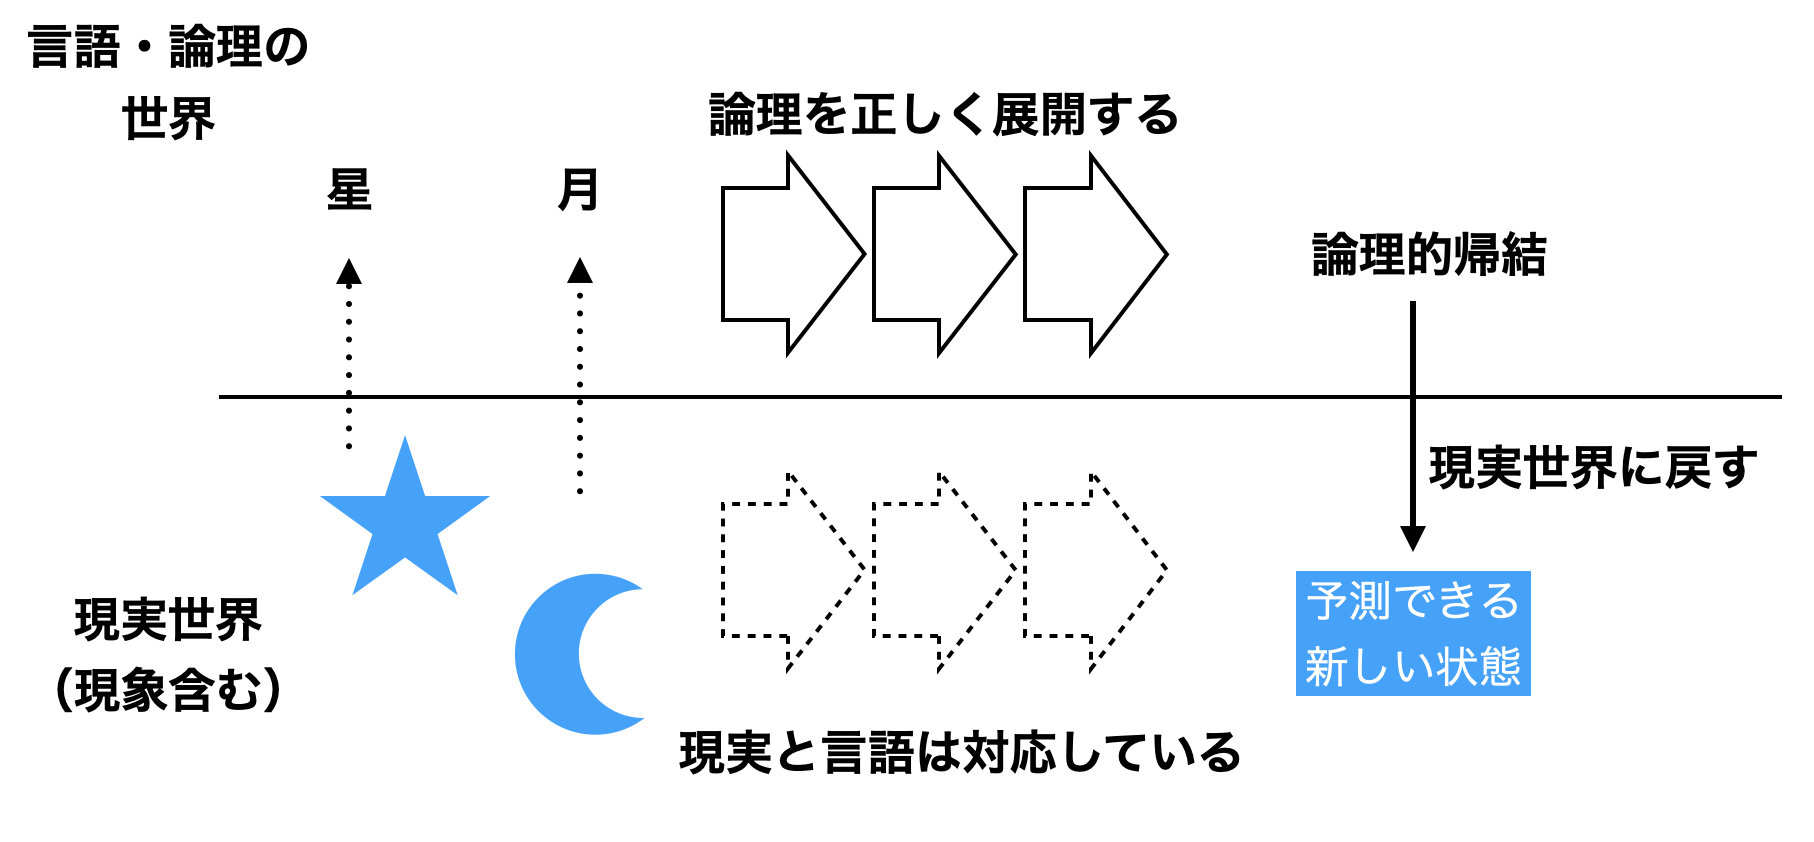
\includegraphics[keepaspectratio,width=1\linewidth]{../images/04Wittgenstein.png}
	\caption{世界と言語の対応・論理実証主義\index[termidx]{ろんりじっしょうしゅぎ@論理実証主義}の哲学的基盤}
	\label{Wittgenstein}
\end{figure}

これが我々の生きている，少なくとも認識的なもののすべてなので，正しく世界を写し込んでいるし，記述できない，語り得ぬものについては沈黙しなければならないわけです。名無しの権兵衛には名無しの権兵衛という名前があるではないか，というような話ですね。違うかな？いや，本当に語り得ぬものについては，言語の世界に入ってきていないものについては，あるいはないものを勝手に言葉で指し示そうとしたって，それは正しくない言葉。

だから彼が哲学の問題を全部解決したと言っているのは，ありもしない，現象にたどれもしない，原始命題に戻れもしないような言葉の表面的な類似性とか，それっぽい論理だけで議論しているのは不毛だよ，と。哲学のそういうのは全部まやかしだ，と喝破するわけです。全部現実との，どこかのレベルで現実との対応があるはずなので，そこがしっかりと結びついているものであれば，論理を正しく運用すれば，世界を全部記述できます。だから哲学の問題は終わり。これがウィトゲンシュタイン\index[nameidx]{うぃとげんしゅたいん@ウィトゲンシュタイン}の考え方なのですね。

言葉と論理で表現できないものがあるのなら，それはもうどうしようもないものだ，ということで，7つの命題の中に，世界の記述の定義から始まって，世界の閉じ方まで書いてある。これで終わっているわけです。

私の解釈が間違っていたり，何か言葉遣いが間違っているかもしれませんから，皆さんぜひこの本を読んでください。私は，「世界は成立することがらの全体である」という，一文だけを一日考えても，反証もなにも思いつかなかったし，何が書いてあるかは分かるけど，何が書いてあるか全く分からないみたいな，いい本なので，ぜひ読んでいただきたいです。

実世界で誰かが何かをこうしたみたいな，実世界のような現実，現象の移り変わりみたいなのも，言葉でしっかり記述(写像)できて，ここには対応関係があるでしょということを言うわけですね。

これが20世紀の頃に，さあ科学をやろうという，近代科学を盛り上げるときのブースターになるわけです。なぜなら，世界がこのような仕組みになっているのであれば，きちんと記述して，論理を進めていけば，将来にどうなるのかというのは，しっかり予測できるでしょう？

現実問題としてこのような現象がありますということを抽象し，どう変わっていくかを論理の上で進めていって，その先で理屈上こうなるという仮説にし，現実と照らし合わせれば，合っているかどうかをきちんとチェックできて，科学としては前進することができる。これが論理実証主義\index[termidx]{ろんりじっしょうしゅぎ@論理実証主義}という考え方の哲学的基盤になるわけです。

ウィトゲンシュタイン\index[nameidx]{うぃとげんしゅたいん@ウィトゲンシュタイン}が，論理実証主義\index[termidx]{ろんりじっしょうしゅぎ@論理実証主義}者を，私の哲学でこうやって研究できると言ったわけではなくて，単純にそれを読んでいた，見ていた人たちが，なるほど，これで科学というのをしっかりと記録，記述できますねというふうに考えたというだけなのですが，少なくとも，この論理実証主義\index[termidx]{ろんりじっしょうしゅぎ@論理実証主義}的に，科学というのは前進するのだというふうな，機運が高まったというわけです。

\subsection{後期の言語ゲーム的発想}
さて，そうではあるのですが，ウィトゲンシュタイン\index[nameidx]{うぃとげんしゅたいん@ウィトゲンシュタイン}はその後，『哲学探究』という本を出します。

彼は『論理哲学論考』という本を書いて，これで哲学の問題は終わりということで，哲学を辞めて田舎に引っ込みます。田舎に引っ込んで，小学校の教師をやったり，お姉さんの家の建築デザインをやったりして過ごしていたのですけれども，その間もずっと考えていたみたいなのですが，休んでいる間に考えていたことは何かというと，この『論理哲学論考』で言っていた話を，全部台無しにするような発想です。

それは何かというと，「言葉というのは，世界を全然映したりしていません」と言うのです。前期のウィトゲンシュタイン\index[nameidx]{うぃとげんしゅたいん@ウィトゲンシュタイン}は，言葉は世界の写像です，という話をしていたのに，後期に入ったら，言葉ってそんなものではないとちゃぶ台返しです。ルールがこうやって決まっているから，こうやって言葉を使うというのではなくて，言葉というのは，その言葉が指し示している意味は，どこにあるかというと，その言葉が現場でどのように使われているかだ，と言うのです。

これを「言葉の意味は，その使用である」というのです。使用というのは使うということです。使い方です。つまり，言葉をいくら繰り返してみたところで，現実にはたどり着きません，という話をするのです。

その『探究』の話の中に入っている，例え話があります。街の中で大工さんが，煉瓦を積んでいる工事をしている。高いところで工事をしている親方が，下にいる若者に，「石板，石板」と言うのです。そうしたら，弟子が分かっていて，「はい，親分」って，さっと石板，煉瓦みたいなものかな，その場に置かないといけない，適切なものを親分に渡す。さて今，親分が，「石板，石板」と言った，その言葉のどこに，「私は今からここに煉瓦を積みますから，適切なサイズの材料を持ってきなさい」というような意味があったか。「石板」という二文字の中に，そういうのは入っていないですよね。

ただし，文脈の中で，その世界の中で，親方が，このタイミングでこういう時に，「石板」と言ったら，この煉瓦をあそこに置いて，今から積み上げていくのだから，持ってこいよという意味だなというのが，弟子には分かるわけです。親方ももちろんそのつもりで言うわけです。つまり，使っている人たちは，その言葉の意味が分かっているわけです。

「石板」という言語をどんなに探しても，その意味とかルールとかは出てこない。我々は言語をこうやって使って，今も講義などやっていますけど，言語って，ではどういうルールなのですか。この『論考』に書いてあったような，論理的なつながりの，どういうルールなのですか。実はそんなルールはどこにもないし，我々は生まれた途端に，言語を使っている。この言葉を使ったゲーム，言語ゲームというのですが，そのゲームの中に放り込まれるわけです。その言語ゲームという中に放り込まれて，いきなりプレイしながら，この言葉の使い方はこういう意味ではないかというのを体得していくしかない。だから，言葉に世界を写す意味なんかないのだ，と彼は言い出すのです。

だから，みんな，「あなた，これでサイエンスができると言ったじゃないか」ってびっくりしたと思うのですけれども，そういうふうな感じで，ウィトゲンシュタイン\index[nameidx]{うぃとげんしゅたいん@ウィトゲンシュタイン}は後期になって，話をひっくり返します。

\subsection{言語哲学と社会心理学の接点}
さて，今言った話，どこが社会心理学と関係あるのか。実は社会心理学の中に，もうまだこの前期の発想は残っているわけですね。社会心理学者はデータを取って，自分の立てた仮説が，しっかりと検証できるかどうかを考えましょう，という論理実証主義\index[termidx]{ろんりじっしょうしゅぎ@論理実証主義}的な発想は，今でも色濃く残っています。

つまり，現象を構成概念にきちんと写像して，それを論理的に考えると，こういうのはこう来てこうなるはずだから，こういう仮説が成り立つはずだ，と考えている。言語の世界でロジックを先に進めて，その結果として予想しうる現象について，データを取ってみて，ロジックの道筋つまり理路が，果たして正しかったかどうかを検証する，というスタイルで，今でも社会心理学の論文は生産されています。そういう意味では，前期ウィトゲンシュタイン\index[nameidx]{うぃとげんしゅたいん@ウィトゲンシュタイン}の発想というのが，今の社会心理学の半分ぐらいを覆っているのです。

もう半分は何かといいますと，言語ゲームです。言葉にそういった意味はない，というような発想から何が出てくるかというと，ナラティブです。ナラティブ的なアプローチですね。社会心理学の中には，言葉の辞書的な意味にとらわれず，その言葉が発せられた人やその人が属するコミュニティにおいて，どんな意味を持って使われたのか，つまり文脈の中でどのように意味が形成されたのかを研究するというやり方も残っています。こうしたより実践的側面も，社会心理学の一領域なのですね。言葉の意味，その界隈での言葉，用語の使われ方としての社会心理学というか，文化的な意味を考える社会心理学。グループダイナミックス\index[termidx]{ぐるーぷだいなみっくす@グループダイナミックス}学会というのは，どちらかというとそちらを指向しました。社会心理学会がどちらかというと，この前期の方を指向した学会として今も残っている，というのが私の見立てです。

グループダイナミックス\index[termidx]{ぐるーぷだいなみっくす@グループダイナミックス}学会がナラティブを扱う社会心理学に傾倒した，という話はまた後で丁寧にいいますが，先に少しだけ触れておきます。ガーゲン\index[nameidx]{がーげん@ガーゲン}という人が，社会心理学というのは歴史学だという論文を書いています。``Social Psychology as History''という論文です\parencite{gergen1973social}。

この論文の主張は，心理学が一見自然科学のように見えるが，実際にはそうではないというものです。具体的には，心のあり方やその時にどのように感じ，何が起こったかということは，すべてその人が生きてきた中での言葉の意味や，それを受け止める社会の中での言葉の使われ方に依存する，という点が強調されています。自然科学の実験のように，何年も前の実験を再現しても同じ結果が得られる，といったものではないのです。たとえば，ニュートン\index[nameidx]{にゅーとん@ニュートン}がボールを落とす実験のように，場所や時刻が違っても，初速度と質量がわかっていれば結果を予測できるといったサイエンスとは異なるのです。心理学は，その意味ではむしろ歴史学に近いと言えるでしょう，とこの論文では主張されています。

そこから社会心理学の中で，社会的構築主義という一派が，ちょっと出てきた経緯もあるんですけども，そういった文脈もあるのだということは，知っておいてください。

要約すると，ウィトゲンシュタイン\index[nameidx]{うぃとげんしゅたいん@ウィトゲンシュタイン}という20世紀の哲学者の考え方によって，社会心理学にも前期と後期の2つの流れが生まれたということです。ウィトゲンシュタイン\index[nameidx]{うぃとげんしゅたいん@ウィトゲンシュタイン}の思想の後には，分析哲学や，言語の分析を中心とした哲学的な動向が発展していきました。また，時代的には言語学も台頭し，これらの動きがほぼ平行して進展していたことも重要なポイントです。そのことと社会心理学の考え方，研究方も無縁じゃない。それどころか，パラレルな関係にありますよね。こうした動きを知っておくと，また理解が深まるかと思います。

あとは，ちょっとだけ，その社会思想のもう1個のルートの話をして，社会心理学の歴史を始めますね。
それは何かと言いますと，構造主義という考え方です。

\section{構造主義の考えかた}
申し訳ありません。今から私が話したいのは構造主義です。レヴィ=ストロースの話がしたい。いけませんね，完全にボロが出ました\footnote{このとき私は何を勘違いしたのか，黒板に大きく「構成主義」と書いてました。}。
\subsection{レヴィ＝ストロースと婚姻規則}
構造主義って皆さんご存知ですかね。私はおそらくですが，構造主義が社会に浸透した頃に生まれてきた人間なのだろうなと思います。1970年代の生まれなのですけれども，レヴィ=ストロースが『親族の基本構造』というのを書いたのが1949年みたいですね。さて，レヴィ=ストロースという人類学者\footnote{クロード・レヴィ＝ストロース\index[nameidx]{れゔぃ＝すとろーす@レヴィ＝ストロース}(Claude L\'{e}vi-Strauss，1908年11月28日 - 2009年10月30日)は，フランスの社会人類学者，民族学者。ベルギーのブリュッセルで生まれ，フランスのパリで育った。専門分野である人類学，神話学における評価もさることながら，一般的な意味における構造主義の祖とされる。(Wikipediaより)}がですね，『親族の基本構造』という本を書きます。

当時それまでの人類学とか民族学というのはどういうことをやっていたかというと，極端な話，未開の世界に出かけて行って変な民族の風習とかを見つけて，帰ってきて報告して，「あんな変な民族がこんな変なことをやっていますよ」という報告をすると，「おもしろい物を見つけてきたな」と言って褒められるという世界だったみたいです。その考え方のもとになるのは，「未開」という言葉にあるように，社会はまだ開けていないという状態から開けているという状態に進んでいきますよという考え方なのですね。

この辺の考え方には，マルクスやエンゲルスの発想も基礎にあります。マルクスの唯物史観というのは，結局のところ，私たちの生活の基盤である「どのように生産し，その生産物を分配・運用していくか」という点に根ざしています。このように，物質的な側面がすべての仕組みの基礎にあり，そこから世の中の成り立ちを考えるわけです。ですから，「唯物」というわけです。物質的な基盤が大きく変わらなければ，新しい発想も生まれず，心情の面もそれに追随しない，という考え方なのです。

原始時代には，人々が共同で農作物を生産し，平和にシェアして暮らしていました。その後，封建時代が到来します。封建時代では，土地を貸し出すことで，自ら働かずとも報酬を得るシステムが確立されました。さらに時代が進むと，個人の私有権が認められ，働いた分だけ報酬を得て収益を上げられるようになります。しかし，そうした時代においても，労働者と資本家の間で富の「使う側」と「使われる側」に分かれる構造が存在し続けました。現実には労働者が物理的に物を動かして生産を行っているにも関わらず，ブルジョア階級はそれを私有し，実際に生産には関与していないのに富を得るという状況が発生していきました。

マルクスとエンゲルスは，歴史がこうした一方向に進む中で，理想的な未来として「ユートピア」が訪れる可能性についても考えました。そのユートピアでは，働きたい人は好きなだけ働いて，その分の報酬を得る一方，働かなくても必要なものを得られる，という社会が実現されるのです。つまり，共同で生産し，共同で富を分け合う社会の到来が予見されている，というのが彼らの思想でした。

ものすごく雑な説明の仕方で，「いや，そんなのではない」と言われたら，もう申し訳ありませんと言うのですけど，少なくとも私はそう理解しているというぐらいでお控えください。本当かなと思ったら皆さんなりに考えてほしいのですが，全部私の創作で話しているわけでもないですし。

少なくともマルクスは，世界がそうやって一方向に進むと考えていた。だからこそ，そのシンパが社会主義革命を起こすわけですよね。今はまだ資本主義の段階で，労働者と資本家というのが分かれているのだけれども，世界は絶対その方向に行くのだから，先にその世界の方を持って来ようというのが社会主義革命なわけです。

そういうふうな唯物史観というものの考え方，社会は少なくとも貧しい状態からだんだん豊かな状態に進んでいくのだという発想が時代的にあったわけです。だからこそ，進んだヨーロッパの人間が未開の土地に行って，進んでいない人を見ると「変なことをしてる」となるわけです。彼らがやっていることは，少なくとも先進国の人から見たら何のためかわからない。つまり，機能的には説明ができないんです。何のためにそれをやっているのかと言われても，全く説明できないようなことを未開の人たちはやっている。ということは，この人たちは劣っているのだから，あるいは社会がまだ未開なのだから，教化して発展させてあげないといけないね，という話にもなりますよね。

それが世界の流れだったわけですね。20世紀の世界の流れで，それが大きな2つの世界大戦を生み，それ以外にもいろいろな大戦や紛争を生んでいるわけなのです。そういった中に出てきたこのレヴィ=ストロースさんが言ったことは何かというと，何のためにやっているかが分からないというのは未開だからじゃないよ，ということです。実は我々が理解できないけれども，ちゃんとそれが意味があることをしているのですよ，彼らなりに意味があることをしているのですよということを言うわけです。

未開の人の側からしたら，「何を当たり前な」と思うかもしれないけれどもですね。でも，劣っているものがだんだん成長して優れたものになっていきます，優れているものは劣っているものを引っ張り上げなければいけません，というような考え方は，それはそれで自然な発想だとも思います。時代的には，未開のところから発展していくという一方向性が自然だったのですけれども，そこに出てきたのが「未開は未開と言うけれども，彼らは我々と同じようなことを違う方法でやっているだけで，彼らなりには意味がありますよ」というようなことを言った構造主義です。

彼が書いてるのが『親族の基本構造』。その前には『野生の思考』という本も書いているのですけど，『親族の基本構造』で扱ってるのは親族，家族関係です。より具体的にいうと，婚姻関係，特にインセスト・タブー\index[termidx]{いんせすと・たぶー@インセスト・タブー}の研究をしています。

皆さん，近親婚は禁止されているというのは知っていますよね。知っていますよねというのもおかしい話ですが，近親婚禁止，つまり親兄弟と夫婦関係になってはいけませんよというようなルールは西洋はもちろんのこと，それこそ未開のと言われたところにもちゃんとあります。

とある部族なんかは，母方のお兄さんから生まれた女の人をお嫁さんに迎えるのは喜ばれるけれども，父方のお姉さんから生まれた女の人をお嫁さんに迎えるのは良くない，というルールがあったりします。「何だそれ」と思うかもしれませんけど，誰が誰と結婚して良くて，誰が誰と結婚してはいけないみたいなのが，ものすごく複雑なルールが世の中にはいっぱいあるわけです。インセスト・タブー\index[termidx]{いんせすと・たぶー@インセスト・タブー}。その子とこの子は婚姻関係を結べないよ，というタブーのルールがいっぱいあるわけです。

これについて，「未開の部族だからそんなことをしているのだろう。おかしな風習だな」と簡単に片付けることもできます。しかし，レヴィ＝ストロース\index[nameidx]{れゔぃ＝すとろーす@レヴィ＝ストロース}が指摘したのは，このルールを守ることで，血縁が濃くなりすぎないように調整されている，という点です。さらに，女性が財として交換され，部族間を巡ることで，男女の人口バランスが保たれ，婚姻が常に平均的に成り立つようになっています。この制約のおかげで，どの部族も滅びることなく存続できる状態を維持しているのです。

さらに。気づかなかっただけで，その親族の婚姻関係の中には，数学的な関係があります。これは群論です。群論というのは，交換の法則だとか，どのように交換したら，群が元に戻るかみたいな，群として閉じているか閉じていないかを考える数学的な学問なのですけれども，親族のその婚姻のルールの中に，今言った基本構造，群が成立しているということを明らかにしたのです。それが，レヴィ＝ストロース\index[nameidx]{れゔぃ＝すとろーす@レヴィ＝ストロース}。正確には，アンドレ・ヴェイユ\footnote{アンドレ・ヴェイユ(Andr\'{e} Weil, 1906年5月6日 - 1998年8月6日)は，フランスの数学者で，20世紀を代表する数学者の一人。架空の数学者ブルバキの中の人のひとり。}という数学者のアイデアです。レヴィ＝ストロース\index[nameidx]{れゔぃ＝すとろーす@レヴィ＝ストロース}は数学のことを全然分かっていなかったという説もあるのですけれども，ともかくこの本で，「構造」を見出したわけです。

つまり，先進国から見て「意味が分からない」と感じることにも，実際には意味があり，たとえその機能的な意味がすぐに理解できなくても，そこには一般的な仕組み＝構造が存在するのです。どうしても先進国の人々は「何のために」「どう機能するのか」といった「機能」の面を重視しがちですが，レヴィ＝ストロース\index[nameidx]{れゔぃ＝すとろーす@レヴィ＝ストロース}は，それよりもまず仕組みが先にあって，その仕組みが機能を裏支えしているに過ぎない，という見方を提唱しました。つまり，機能が分からないからといって，その仕組みが無意味だとか機能していない，というのは間違いだと述べたのです。

\subsection{構造主義から見る社会変容}

こうした考え方が，「人間関係や社会を機能ではなく，構造から見ましょう」という発想を生み出しました。言い換えれば，世界はただ一方向に進んでいるわけではなく，どの社会にも共通する構造があり，それが異なる見え方をしているに過ぎない，という考え方です。

なぜこのような考え方を強調するかと言えば，この思想が日本社会にも深く浸透し，現在では2世代，3世代にわたって定着しているためです。皆さんのような若い世代からすると，昔の話を聞いて「なぜそんなおかしなことをしたのだろう」と思うことも多いかもしれませんが，私が子供だった頃には，例えばランドセルの色が完全に決まっていて，女の子は赤，男の子は黒という二択しかなかったのです。

昔の人々は，「男の子とはこうあるべき」「女の子とはこうあるべき」という考え方を強く持っていました。その価値観において，男性の中でも「優れた男性」と「劣った男性」が明確に区別され，上下関係や前後関係がはっきりしていたのです。そして，「いつか自分も大人になって，男性ならこうなる，女性ならこうなるべきだ」という期待があったのです。しかし，私が親になった何十年か前には，すでに子どもたちのランドセルの色も多様化してました。私が子どもの頃には黒しか選べなかったランドセルも，個性を重視する時代になっていったのです。

その走りが，私が子供の頃の雰囲気かなと思ってます。ちょうど学校の先生が「個性が大事」と言い始めた時代でもありました。「個性が大事」とはどういうことでしょうか。つまり，一人ひとりの考え方ややり方が尊重されるべきだ，という話ですよね。例えば，勉強が苦手に見える子や足が遅い子も，彼らなりに努力しており，それぞれの環境や制約の中で頑張っているのです。みんなが同じ形で頑張るのではなく，それぞれの「心持ちの持ち方」も含めて多様性を認めよう，という考えが1980年代頃から広まりました。このような姿勢は，構造主義的な発想が個人レベルにまで浸透してきたからではないかと私は考えています。

今や，「人それぞれ事情がある」「多様性の時代である」といった考え方が一般常識となり，他者を否定せずお互いを尊重するのが「マナー」として根付いています。構造主義的な視点から見ると，たとえ一見機能的に劣っているように見える場合でも，実は同じ仕組みが働いていると考えるからです。そして，この「考え方」が現代に受け継がれているのです。ちょっと強調しておきたいのは，そんなに遠い昔の話じゃないということです。私の子供の頃といっても50年も前じゃないですよ。皆さんが今，当たり前だと思っている考え方も，最近の社会思想が市民の手元に降りてきて，常識化した結果であり，2世代と前の話じゃないんです。

構造主義とは，優れているとか劣っているという評価を絶対的なものとせず，見た目の問題ではなく，根底にある仕組みが皆同じであるという考え方です。「みんなそれぞれ事情がある」「それぞれ頑張っている」という発想もここから始まります。構造主義が成熟し，やがてポスト構造主義やポストモダニズムといった新しい思想が登場しました。社会思想として見れば，現代はすでにポスト構造主義のさらに先の時代にあります。2024年の今，個性や多様性が重要であることは当たり前のこととなり，「個性が大事だ」とわざわざ言う必要もないほどです。しかし，50年ほど前の時代には，皆が同じであることが当然視され，「優れている」「劣っている」という評価基準も明確に存在していたのです。

社会的な思想はわずか50年ほどでも大きく変わり，まったく異なるものになることがあります。昭和の頃の話を聞くと，「努力と根性で乗り越える」といった非科学的な価値観が強かったように見えるかもしれませんが，当時はそれなりの合理性があったのです。この発展は，例えばマルクス的な理論によるポジティブな方向への進化であったり，レヴィ＝ストロース\index[nameidx]{れゔぃ＝すとろーす@レヴィ＝ストロース}のように「発展というよりは，どのレベルでも同じ仕組みがある」という見方であったりします。構造主義は，言語学などの分野とも深く結びつき，世界の捉え方に大きな影響を与えてきたのです。

言語学，あるいはそれを一歩進めたカルチュラル・スタディーズ\index[termidx]{かるちゅらる・すたでぃーず@カルチュラル・スタディーズ}みたいな思想がその後出てきます。もちろん先ほど言ったナラティブ，言葉による世界の切り取り方，作り方みたいなものも関係してくるんですけど，こういったアイデアが現代に影響してるんですよ。あるいは皆さんの日常的な感覚というのも，社会思想的な潮流が何十年かたって浸透してきているのだ，と考えてみてください。別にレヴィ＝ストロース\index[nameidx]{れゔぃ＝すとろーす@レヴィ＝ストロース}が構造主義の本を書いたから小学校の先生が「個性が大事」って言い出したという直接な因果関係があるわけではないのですけど，社会的な考え方のムーブメントといいますか，発想のノリですね。そういうのって本当に時代とともに大きく変わるのですよ。

それこそ歴史なんかを勉強されている方は，その辺を想像するのが楽しいのではないかなと思ったりします。例えば古代ギリシャの研究とか振り返ると，ギリシアの時代は例えば同性愛が普通だったんですよね。ギリシャは男性同士の同性愛が良いこととして認められていた，というのはよく知られています。日本でも戦国の時代なんかも同性愛がありふれていた，って言いますけど，こんな性の歴史を一つ取ったとしても今の我々の感覚とちょっとでも時代が違えば雰囲気は全然違うわけです。

そういった状況を理解するためには，まずその時代を構成していた考え方とか発想みたいなのが必ずバックボーンにあるからなので，その辺をイメージしながら，「では社会心理学というのはどういうふうにして生まれてきたのでしょうね」という話に進んでいきたいと思います。

\section*{いんたーみっしょん：今週の推薦図書}

はい，ここで少し時間を取って，本の説明・紹介をしておきたいと思います。ウィトゲンシュタイン\index[nameidx]{うぃとげんしゅたいん@ウィトゲンシュタイン}に関しては様々な解説書もありますが，解説書などを読むよりは『論理哲学論考』や『哲学探究』という彼自身が書いている本に一度触れていただきたいと思います。この7つの命題だけで全てを書き切るという，その意気のよさ。そして言葉の端々にまで当然のことながら，非常にこだわりもって作られています。たった7つの命題，もちろん下位命題はもっと多くありますが，7つの命題の中に世界を全て埋め込もうとしているわけですから，非常に丁寧な書き方をしています。『論理哲学論考』，『哲学探究』については原典に当たられることをお勧めします。

構造主義に関しては，私は橋爪大三郎という方が書いた『初めての構造主義』\parencite{Hasidume1988}，これは講談社現代新書なのですが，これが読みやすかったと思います。

もう少し数理的に進みたい，あるいは理論的に深く理解したいという方は，ちくま学芸文庫に出ている『思想の中の数学的構造』\parencite{MasoYamashita2006}，これは非常に興味深い本です。『思想の中の数学的構造』という書名が示すように，我々が物事を考える際の言葉の背後に，例えば「当たるも八卦，当たらぬも八卦」の八卦の話なども含まれていますし，冒頭はレヴィ＝ストロース\index[nameidx]{れゔぃ＝すとろーす@レヴィ＝ストロース}の基本構造のところから始まるのですが，このような数学的な発想が実は我々の考え方の中にビルトインされているという話があり，興味深い内容となっています。

それから，構造主義，つまりみんな何の役に立つか立たないかだけで考えるのではなくて，その機能ではなくて構造の方を見ましょうねというふうなこと，つまり構造的には同じことをやっていますよ，みんなそれぞれなりの仕組みがありますよという考え方。これは私はとてもリベラルで現代的だし，その中で育ってきたからそう言っているだけかもしれませんけど，とても自然な発想かなと思うわけですけれども，この構造主義の後にポスト構造主義というのが出てきます。デリダ\index[nameidx]{でりだ@デリダ}とかドゥルーズ\index[nameidx]{どぅるーず@ドゥルーズ}とかですね。先ほどちょっとカルチュラル・スタディーズ\index[termidx]{かるちゅらる・すたでぃーず@カルチュラル・スタディーズ}って言いましたけど，そういう人たちが出てきます。その人たちは意味とか悪いとかではないのだ。構造が整っていればいいのだ。それをちょっと飛び越えて，もう何でもいいから面白かったらいいのだ。それらしい言葉で，それらしいことを言っていればそれらしいのだっていう考え方かと思います

すごいふわっとした説明で申し訳ないのですが，興味がある人は皆さん，「ソーカル\index[nameidx]{そーかる@ソーカル}事件」というので調べてみてください。『知の欺瞞』という本があります\parencite{chinogiman}。これは，カルチュラル・スタディーズ\index[termidx]{かるちゅらる・すたでぃーず@カルチュラル・スタディーズ}という構造主義以降に登場した流行で，専門用語をそれっぽく組み合わせて深遠な議論をしているかのように見せかける行為があるんですが，それを批判した話ですね。

みんなそれっぽい専門用語で，現代思想について議論している雑誌があるのですが，そこにこのソーカル\index[nameidx]{そーかる@ソーカル}という人が，とある論文を提出します。それはもう最先端の科学用語を，ふんだんに散りばめて，それっぽい議論をしているみたいな内容。その論文が，なかなかまた新しい言葉遣いで面白いことを言う人が出たということで，その雑誌に掲載されるわけです。その提出された論文について，「彼はいいことを言っている，これはああでこうで，それはこうでこうで」みたいな，人々が盛り上がりがあった後で，著者本人が，「私はそんなつもりで書いてないけど，あの論文全部ギャグですけど何か」と言った，という話ですね。それっぽい用語を使って，適当に論文調にしているだけで，「私は何の意味もないことを言っているのに，あなたたちはそれをまじめに議論して，現代思想をやっていますってどういうことだ」，という。

この事件が何がいいのかというと，もう一方向的な価値観というのはないのだから，みんな違うことをみんなバラバラに好きかって言っていたり，あるいは構造の雰囲気が近かったら，一方は物理学の専門用語であったとしても社会学に持ってきたって，栄養生物学の専門用語を化学に持ってって，それとそれとを結びつけて金融の話題を議論してもいいし，みたいな，構造がそれっぽかったら全部まとめていいだろうみたいな，行き過ぎた構造主義みたいなのを批判した，というところですね。構造がそれっぽいから，「っぽい」って言うだけで話していいってわけではないでしょう，科学ってそういうものではないでしょうということを言った一連の話なのですけれども，皆さんもちょっと考えてみてください。

心理学者だって，心理学用語を作って，それで心理学者だけで分かるような言葉遣いで議論を構築しています。理論体系を作っています。どこがギャグではないのですか，というようなことは，痛烈な批判として成立し得るんですよね。社会心理学で仕事をする心理学者もどこか頭の片隅に入れておかないと，失礼なことになるような気がするのですよね。

\section{社会心理学の歴史；準備期}
今日はね，ウィトゲンシュタイン\index[nameidx]{うぃとげんしゅたいん@ウィトゲンシュタイン}の『論理哲学論考』，言葉の話と構造主義の今みたいな話をしてから，社会心理学の歴史の話に入ろうと思ったら，あと20分くらいしかなくなってしまいました。申し訳ありません。社会心理学の歴史をそれでは，準備期というところで，ちょっと話を始めたいと思います。

ここでも話し尽くせないところがいっぱいあるのです。『アナトミア社会心理学』というテキストで，歴史のところは，6章，「社会心理学の歴史」というのがあって，それのセクション2が「社会心理学の準備期」というのがあります。そこに書いてある話題について，ちょこっと触れていきたいと思います。

\subsection{群衆のパワー}

今言ったように，今からやっと社会心理学の授業を始めるわけですが，科学の考え方とか，人文社会科学の考え方とか，社会思想みたいなのが，どういうふうな雰囲気になっていたかということが重要です。科学の中にある社会心理学，その中にある社会心理学の課題が，どういう状況から出てきたか。社会心理学なんて20世紀の途中になってから，急に盛り上がってきた学問ですからね。学問としてはすごい若い方だと思うのだけれども，それがなぜ成立したのかということを考えると，そういった時代の雰囲気みたいなの，避けて通るわけにはいかないからですよ。特に社会心理学というのは，そのそもそものスタートは，人文学，人類学，民族学，社会学みたいなあたりから，生まれてきているものですから，その辺の時代背景というのを踏まえておきたいと思います。

主に話のスタートはヨーロッパからになります。アジアのあたりがどうだったのかということについては，十分触れられません。すみません。最近はそういうところもしっかりやろう，という学問があるらしいんですけどね。一応，近代科学ですから，ヨーロッパの方から始めていきます。

さてそうすると，私もヨーロッパの人間ではないから想像するしかないのですけど，やっぱり産業革命とかフランス革命というのはすごかったみたいですね。どうしても私なんかは，歴史の授業を真面目に受けていませんでしたから，フランス革命がありました，産業革命がありましたと言われたら，「そうですか」でおわっちゃう。産業革命によって機械化が進んだのですねとか，フランス革命によって王様が殺されたのですね，と情報として受け止めてしまいますね。今年のパリオリンピックで開会式の時に，フランス革命の時の貴族が首を切られたシーンを模したようなオープニングがあって，物議を醸していましたが，フランス革命というのはやはりフランスの精神を代表する，フランス人にとっては誇るべき歴史的出来事なのでしょうね。

でもまあ，当然のことながら，単にフランス革命が起こって，王様が処刑されましたよ，これで民主化というか，市民が生まれましたよ，という単純な話ではないんですね。フランス革命ってその後も何十年も続く長い話の入り口であって，その後にもナポレオンとかで皇帝が戻ってくる時代みたいなのがあったりして，いろんな紆余曲折があったわけです。

ただキリスト教，あるいは教会の中心主義みたいなのは，弱体化していったんでしょうね。そのあと，特に国民意識の誕生とかというのは，第一次世界大戦の頃になりますが，これも大きな「生きてる人間の感覚」がかわったところでしょう。つまり国家というものが出てきて，その単位で国のために戦うぞとかというのが出てきたから，戦争というのが話がややこしくなったわけです。

それまでの戦争というのは，王様と王様，貴族同士の喧嘩であって，貴族同士の農民を守るためのガードマン同士の喧嘩です。これはもう勝ち目がないなとか，儲けにならないなと思ったら戦争は終わるのですけれども，国民とか民族みたいなのを単位にしてしまうと，何というのか，本当に，総力戦になってしまうというのが，戦争の20世紀に我々が体験した戦争の恐ろしいところなわけですね\footnote{この辺りの話は，コテンラジオ\url{https://coten.co.jp/services/cotenradio/}というネットコンテンツがソースになってます。コテンラジオは，学校では教えてくれない歴史をラジオで面白おかしく伝えてくれるもので，最近私は通勤途中に聞いてます。知的興奮が好きな人には超オススメですよ。}。

国民国家というのが生まれたことによって，その土地，その国に生まれた人が全員戦うようなソルジャーになってしまうわけです。社会心理学として大事なのは，その時にやっぱり，市民革命だとか，大きな世界大戦とかをやった，あるいはその中で生きていた人間が驚いてるということ。人間がこんなこともしてしまうのか，とやってる当人たちでも思うわけですよね。

近所の仲のよかったパン屋さんと暴動で一緒に棒を持って声を上げる，みたいなことがあったりするわけです。もちろんそれを「あったりするわけです」とか言っている人も，たぶん興奮して一緒になってやっていたのだと思うのだけれども，そのとき群衆というのは，人というのが集まるととんでもないパワーを生み出すのだな，ということは誰でも分かるわけですね。

これをちょっと引いた目線，アカデミックな目線で見ると，群衆とリーダーとか，それをどうコントロールするかという問いにつながります。特に第二次世界大戦ナチスの頃はプロパガンダと言って，どのように国民に情報を与えて，戦意を盛り上げるか，みたいな話を，当時の政治主体が考えてたわけですよね。

それもちょうどマスコミュニケーション\index[termidx]{こみゅにけーしょん@コミュニケーション}の手段が発展してきたというのとも相まっているわけなのですけれども，そういった大衆が生まれる，それをどうコントロールするか，大衆のパワーとはどれぐらいのものか，というのが考えるべきテーマになってきた。大量生産，あるいは機械化することによって，人間が疎外感を抱く。隣の人が何する人かも分からないような，小さなコミュニティでみんな顔の見知りの世界から都市ができる。働きに出かけたそこの工場で仲間はできる，でも隣の人は何をしているか分からないみたいな，そういうような世界が，それまでなかった状況が出てきた。そこで，そういうたくさんの人のパワー，気持ち，心ってどうなっているんだ，という学術的な問いみたいなのが，そもそもの社会心理学のスタートなのだろうと思うわけです。

\subsection{「大衆」の学術的な位置付け}
ヴント\index[nameidx]{ゔんと@ヴント}という人が，ライプチヒ大学に心理学実験室を作りましたよ。これで実験心理学というのはスタートしていて，心理学は哲学から分離してスタートしましたよということを言いますけれども，ヴント\index[nameidx]{ゔんと@ヴント}は晩年，民族心理学\index[termidx]{みんぞくしんりがく@民族心理学}という本を書いてます。

なぜ実験心理学からそっちにいったんでしょうね。おそらく，心の状態というのを実験室で聞いていてもいいけれども，それでは本当にその人の気持ちというのは分からなくて，その人がどういう生まれで，どういう生育環境で，心というのを持っているのかみたいなのを，やっぱりそういう生の生活みたいなのを観察しないと分からないよねということになったからでしょうね。人間のこころというのは何？と言ったときに，社会的な状況みたいなのを考えないといけないなという学問の芽が，20世紀になったら生まれてくるわけですね。

ヴント\index[nameidx]{ゔんと@ヴント}が今言ったような感じなのですけれども，もう一つ有名なのはフランスのル・ボン\index[nameidx]{る・ぼん@ル・ボン}です。このひとが「群衆心」という言葉を提唱します。革命とか，市民運動，民衆の暴動みたいな，人が集まったとき，人は一人一人の思考判断能力を失ってしまう，というんですね。群衆心という``みんなが考えている気持ち''に乗っ取られて，全体としての有機的な一体感を持つのではないか，というわけです。この辺の発想も，社会心理学の芽になっているのだろうな。

\subsection{フロイドの社会心理的側面}

ちなみに，集団的な心といえば，フロイト先生\footnote{ジークムント・フロイト(Sigmund Freud，1856年5月6日 - 1939年9月23日)は，オーストリアの心理学者，精神科医。神経病理学者を経て精神科医となり，神経症研究，自由連想法，無意識研究を行った。精神分析\index[termidx]{せいしんぶんせき@精神分析}学の創始者として知られる。心理性的発達理論，リビドー論，幼児性欲を提唱した。(Wikipediaより)}も関係してきます。フロイト先生は，無意識を「発見」した人ですね。フロイト先生の無意識というのは，非科学的だと思われるかもしれませんけど，実はすごく科学的なアイデアなんです。

我々が意識していることというのはもちろんあるのですが，人間には生のエネルギーがあって，このエネルギーに突き動かされて，人というのは生きるのです。このエネルギーをリビドーとかエスとかというわけですけど，生きるためのエネルギーがベースにあって，この力で我々は精神活動をやっていると考えます。これが特に快楽原理に基づいているとか，全部性的なところで説明する点に問題があります。全部性的，というのを「汎性説」というんですが，そこにつながるからフロイト先生は嫌われるというか，ちょっと変態っぽく言われてしまいますね。

この生きるためのエネルギー，生命のエネルギーみたいなのがあって，これを発露させたい，というのが人間。ただし，快楽原理に従って生きるためのエネルギーを全部ばらまいてしまうと，要は，もうなんていうのか，獣と同じなわけです。例えば，ここで私が急に服脱ぎ出して，性的なことをしたいと言い出したら，そこですぐ捕まりますけれども，そうはせずにちゃんと私，服着て授業しているでしょう。これはなぜかというと，そういうことをやったらダメですよ，というスーパーエゴが働いてるからです。超自我とかも言ったりしますが，そういうことはやったらダメだろうという理性的なものが上から押さえつけているので，社会というのが成立しているわけですね。

このスーパーエゴと生のエネルギー，このエネルギーがぶつかっているところが自我だ，と言われています。ここが我々の持っている自我であって，本当は生きるためのエネルギーというのが，腹の底から湧き出しているはずなのだという人間の「モデル」です。合っているかどうか分からないけど，これ，彼のフロイド\index[nameidx]{ふろいど@フロイド}の考え方は人間のモデルです。

この下からのエネルギーは常に出てこよう，出てこようとしているのだけれども，全部噴出させたらやばいことになるから，押さえ込むわけですね，上から。この押さえ込んでいるのが何かというと，そんなことやったらいけないでしょうという社会性であるし，もう一つはお父さんですね。そんなことやっちゃダメよというような社会，お父さん，理性，ルールみたいなのがぐっと押さえ込むわけです(図 \ref{Freud})。

\begin{figure}[ht]
	\centering
	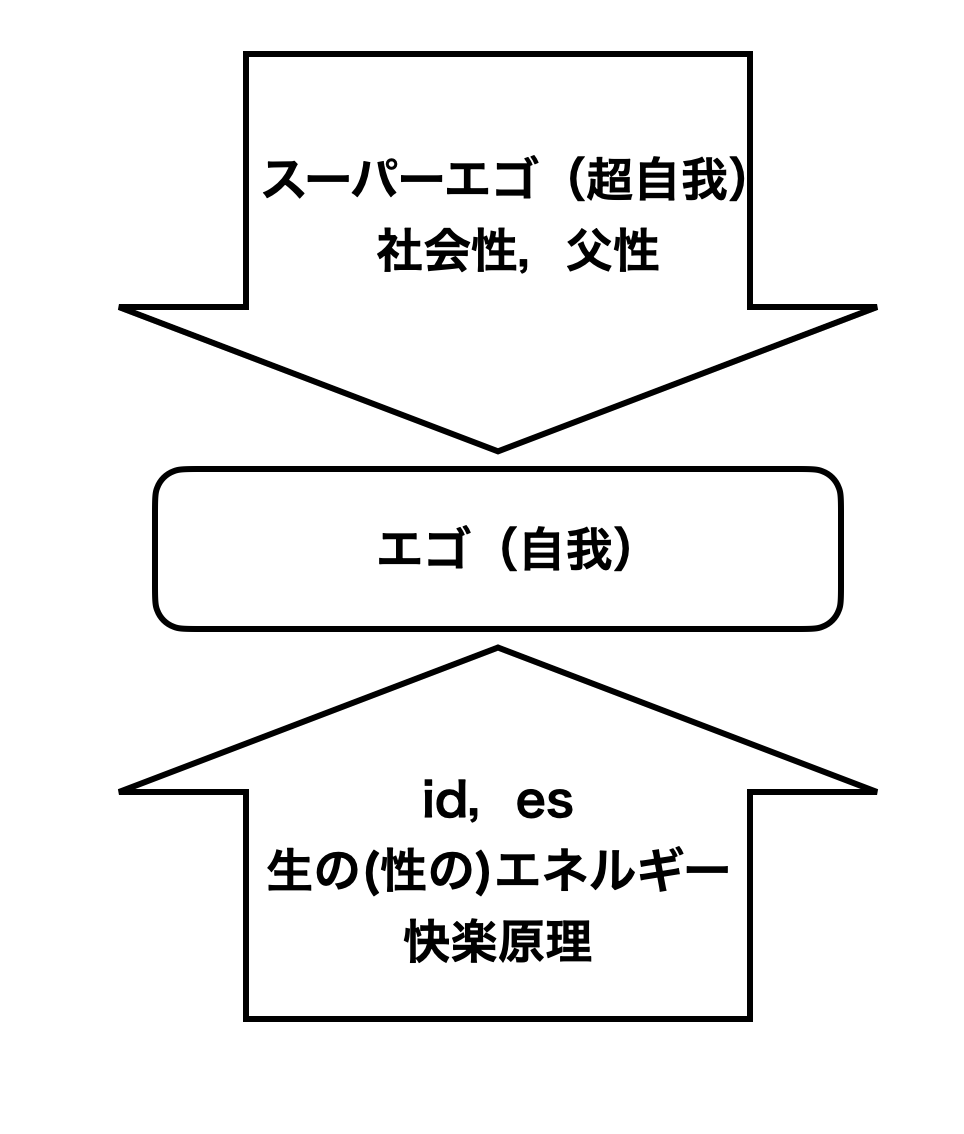
\includegraphics[keepaspectratio,width=0.5\linewidth]{../images/04Freud.png}
	\caption{フロイド\index[nameidx]{ふろいど@フロイド}のモデル}
	\label{Freud}
\end{figure}
さて，押さえ込んで表に出せなかったエネルギーが地下に潜ります。それが無意識です。で，我々は無意識に出てきてはいけない性のエネルギーを押さえ込んでいるのだけれども，それが十分に適切な形で管理，コントロールして押さえ込んでおかないと，ヒステリーのような変な形で出てきますよというのがフロイトの治療の論理なのです。

このモデルが合っているかどうかは，これで患者を治療しているので，治ったかどうかで評価するのも一つの方法ではありますよね。ただ真のモデルかどうか，つまり，そんなにその性のエネルギーが，快楽のエネルギーがあるのか，と言われると，それは分かりません。それはニュートン\index[nameidx]{にゅーとん@ニュートン}が重力を見つけたというのではなくて，このように力関係を記述すれば物理法則が立てられるって言ったのと一緒で，人間の病理というのはこういうモデルで記述すると解釈できますって言ったのがフロイト先生の功績だと思いますから，真実かどうかではなくて，こういう説明体系がありますよということは言っておきたいと思います。

フロイト先生は，もともとは精神症から入っている。身体はどこも悪くないのだけれども，いろんな異常な行動をしてしまいますとか，急に意識を失って倒れ込んだりしてしまいますとか，そういうような臨床的な問題についての説明原理として精神分析\index[termidx]{せいしんぶんせき@精神分析}を作り上げた。これにしたって20世紀の頃という背景があります。すごく近代化が進んで，女性は貞淑でなければならない，男はこうでなければならないみたいな価値観がすごく社会的にはっきりしていた時代なんです。つまりこのスーパーエゴの方がすごくはっきりしていたからこそ，グググッと抑圧するパワーも強くて，こういうモデルが成立した，あるいはこのモデルに基づく治療法というのが成立したのかとも思います。

つまりフロイト先生が，「それってあなたが子供の頃に抱え込んだ性的な気持ちですね」と社交界では超タブーとされるような発言をすると，びっくりするのだけれども，そのことによって何かスーパーエゴがちょっとでもほぐれたら，病状が変わるみたいなことがあったのではないでしょうか。実際にフロイト先生はそれで人をケアしているわけですから，正しいか正しくないかという真実がどうかのゲームは置いておいて，こういうふうな発想があるということだけは，お伝えしておきます。

さて，フロイト先生もこのスーパーエゴというところに社会を見出しているわけですね。彼は臨床で個々のケースについての発想の人ですから，どちらかというと父親らしさ，父親というのは社会の代弁者，ルールの代弁者みたいな感じで子供には映るというふうな説明をするわけですけれども，この社会というのがあるだろうという意味では，心理学における社会心理学の芽の一つでもあるわけです。

ちなみにフロイト先生のお弟子さんのユング\index[nameidx]{ゆんぐ@ユング}先生は，このイドというのが，実は精神世界ではみんなつながっていて，人類みんなつながっているという，ちょっとオカルトチックな説明をします。ユング\index[nameidx]{ゆんぐ@ユング}派の考え方は，私もちょっとよく分かりません。フロイト先生の方がまだ発想としては，そういう言い方もあるかなというぐらいの意味では分からなくはないです。

\subsection{ジェイムズの「心理学」}

そしてもうひとつ，ウィリアム・ジェームズ\index[nameidx]{うぃりあむ・じぇーむず@ウィリアム・ジェームズ}\footnote{ウィリアム・ジェームズ\index[nameidx]{うぃりあむ・じぇーむず@ウィリアム・ジェームズ}(英語: William James, 1842年1月11日 - 1910年8月26日)は，アメリカ合衆国の哲学者，心理学者である。意識の流れの理論を提唱し，ジェイムズ・ジョイス『ユリシーズ』や，アメリカ文学にも影響を与えた。パースやデューイと並ぶプラグマティストの代表として知られている。著作は哲学のみならず心理学や生理学など多岐に及んでいる。心理学の父である。(Wikipediaより)}という人の話をして今日は終わりにしたいと思います。

ウィリアム・ジェームズ\index[nameidx]{うぃりあむ・じぇーむず@ウィリアム・ジェームズ}という人が，``The Principles of Psychology''という本を書いています\parencite{WJames}。日本語では，今田寛先生が訳された「心理学」の上下巻，これも岩波文庫にあるので，興味がある人は読んでみてください。今読んでも面白いことがいっぱい書いてあります。この``The Principles of Psychology''という本は，アメリカ心理学界では教科書として，古くから使われていたものなのです。

そこには意識とは何であるかとかで，心のスタートについての話をいろいろ書いてあるのですが，ウィリアム・ジェームズ\index[nameidx]{うぃりあむ・じぇーむず@ウィリアム・ジェームズ}さんはなかなか面白いことを言ってる。自分の心，自己，自分というのは，自分の中にあるものだけではないよ，というんですね。あの人は他己というのを考えるのです。相手の中にいる自分のイメージ。こういうのも考えて，社会的な自己のあり方みたいなこと提唱します。

この辺は，G.H.ミード\footnote{ジョージ・ハーバート・ミード (George Herbert Mead，1863年2月27日 - 1931年4月26日) は，アメリカの社会心理学者。哲学者，思想史家でもある。研究業績の多くを，シカゴ大学で行い，プラグマティズムの重要な一人として知られている。ミードは，シンボリック相互作用論\index[termidx]{しんぼりっくそうごさようろん@シンボリック相互作用論}の父として知られている。プラグマティズムの大家，ジョン・デューイとの共同研究も知られている。(Wikipediaより)}の象徴的相互作用論\footnote{またはシンボリック相互作用論\index[termidx]{しんぼりっくそうごさようろん@シンボリック相互作用論}(Symbolic Interactionism)。人間間の社会的相互作用(相互行為)，特にシンボリックな相互作用(symbolic interaction)を主たる研究対象とし，そうした現象を「行為者の観点」から明らかにしようとするもの。(Wikipediaより)}とも関係しますね。ミードの考えた話というのは，頭の中で人間関係のイメージ，象徴，シンボルを相互にやりとりし合いますよねという人間関係論なんです。この辺はミードさんの『精神・自我・社会』という本\parencite{GHMead}を読んでくれれば，ぼんやりと書いてあります。私が読んだけど，はっきりとは分からなかったのですけど。とにかく，そういうふうな考え方があるのですが，それとも似ています。

つまり何かというと，自己というのは，自分の中にあるものだけではないですよという発想です。他人の中にも自己がありますよ。例えば，私は小杉という人間がどんな人間かという自分に対するイメージをもちろん持っていますが，家に帰ると妻がいるので，妻は小杉考司という人間がどんな人間なのかという私のイメージを持っているでしょう。その妻の中にある私のイメージというのは妻が持っているものなのですけれども，私の一部なのですよ，というふうな説明をします。

当然私には子供が3人いますので，子供それぞれの中に小杉考司のイメージがあると思います。自分の持っている自分のイメージもあるけれども，他人に預けている自分のイメージもある。当然私も妻や子供ってこんな人間だろうというイメージを持っていますから，私も彼ら彼女らの自己を預かっていますが，人間関係というのはそういうふうにできているよという説明をしたのがウィリアム・ジェームズ\index[nameidx]{うぃりあむ・じぇーむず@ウィリアム・ジェームズ}さんです。

ジェームズさんのすごく素敵な名言があるので，そこだけ読み上げておきます。

\begin{quote}
    一人の人は彼を認め，彼のイメージを心に抱いている個人の数と同数の社会的自己\index[termidx]{しゃかいてきじこ@社会的自己}を持っていく。これら彼のイメージのどれを傷つけても彼を傷つけることになる。(中略)
人が持っている最も特別で特異な社会的自己\index[termidx]{しゃかいてきじこ@社会的自己}は，彼が愛する者の心の中にあるものである
\end{quote}

素敵ですね。ジェームズさんがその心理学の話の初めで，人間の心というのを考えるときに，他者の中にある自分，他者とのつながりというのを考えないわけにはいかないですよ，というところからスタートしています。

このあたり，まずは社会心理学会みたいなのが成立する前の話ですよ。社会心理学で学問が成立する前なのですけど，いろんな心理学者が，人が集まったら集団心というのがあるのではないだろうか，社会というのは社会のルールというのがあるのではないだろうか，他人の間にも他人の中に自己，他者というのがあって，それの相互作用が社会を作っているのではないだろうかというような，社会心理学の萌芽があちこちにありました。それが20世紀の最初の頃にありましたよ，というところを触れておきたいと思います。

そこから学問として成立するのは来週以降にいたしましょう。申し訳ありません，ほんの入り口しか行きませんでしたけれども，今日の話はここまでにしておきたいと思います。皆さんお疲れ様でした。



\end{document}
